% Options for packages loaded elsewhere
\PassOptionsToPackage{unicode}{hyperref}
\PassOptionsToPackage{hyphens}{url}
\PassOptionsToPackage{dvipsnames,svgnames,x11names}{xcolor}
\PassOptionsToPackage{space}{xeCJK}
\documentclass[
  10pt,
]{article}
\usepackage{xcolor}
\usepackage[margin=0.7in]{geometry}
\usepackage{amsmath,amssymb}
\setcounter{secnumdepth}{-\maxdimen} % remove section numbering
\usepackage{iftex}
\ifPDFTeX
  \usepackage[T1]{fontenc}
  \usepackage[utf8]{inputenc}
  \usepackage{textcomp} % provide euro and other symbols
\else % if luatex or xetex
  \usepackage{unicode-math} % this also loads fontspec
  \defaultfontfeatures{Scale=MatchLowercase}
  \defaultfontfeatures[\rmfamily]{Ligatures=TeX,Scale=1}
\fi
\usepackage{lmodern}
\ifPDFTeX\else
  % xetex/luatex font selection
  \setmainfont[]{Arial}
  \setmonofont[]{Consolas}
  \ifXeTeX
    \usepackage{xeCJK}
    \setCJKmainfont[]{Microsoft YaHei}
  \fi
  \ifLuaTeX
    \usepackage[]{luatexja-fontspec}
    \setmainjfont[]{Microsoft YaHei}
  \fi
\fi
% Use upquote if available, for straight quotes in verbatim environments
\IfFileExists{upquote.sty}{\usepackage{upquote}}{}
\IfFileExists{microtype.sty}{% use microtype if available
  \usepackage[]{microtype}
  \UseMicrotypeSet[protrusion]{basicmath} % disable protrusion for tt fonts
}{}
\makeatletter
\@ifundefined{KOMAClassName}{% if non-KOMA class
  \IfFileExists{parskip.sty}{%
    \usepackage{parskip}
  }{% else
    \setlength{\parindent}{0pt}
    \setlength{\parskip}{6pt plus 2pt minus 1pt}}
}{% if KOMA class
  \KOMAoptions{parskip=half}}
\makeatother
\usepackage{longtable,booktabs,array}
\newcounter{none} % for unnumbered tables
\usepackage{calc} % for calculating minipage widths
% Correct order of tables after \paragraph or \subparagraph
\usepackage{etoolbox}
\makeatletter
\patchcmd\longtable{\par}{\if@noskipsec\mbox{}\fi\par}{}{}
\makeatother
% Allow footnotes in longtable head/foot
\IfFileExists{footnotehyper.sty}{\usepackage{footnotehyper}}{\usepackage{footnote}}
\makesavenoteenv{longtable}
\usepackage{graphicx}
\makeatletter
\newsavebox\pandoc@box
\newcommand*\pandocbounded[1]{% scales image to fit in text height/width
  \sbox\pandoc@box{#1}%
  \Gscale@div\@tempa{\textheight}{\dimexpr\ht\pandoc@box+\dp\pandoc@box\relax}%
  \Gscale@div\@tempb{\linewidth}{\wd\pandoc@box}%
  \ifdim\@tempb\p@<\@tempa\p@\let\@tempa\@tempb\fi% select the smaller of both
  \ifdim\@tempa\p@<\p@\scalebox{\@tempa}{\usebox\pandoc@box}%
  \else\usebox{\pandoc@box}%
  \fi%
}
% Set default figure placement to htbp
\def\fps@figure{htbp}
\makeatother
\setlength{\emergencystretch}{3em} % prevent overfull lines
\providecommand{\tightlist}{%
  \setlength{\itemsep}{0pt}\setlength{\parskip}{0pt}}
\usepackage{bookmark}
\IfFileExists{xurl.sty}{\usepackage{xurl}}{} % add URL line breaks if available
\urlstyle{same}
\hypersetup{
  colorlinks=true,
  linkcolor={Maroon},
  filecolor={Maroon},
  citecolor={Blue},
  urlcolor={blue},
  pdfcreator={LaTeX via pandoc}}

\author{}
\date{}

\usepackage{float}
\usepackage{needspace}
\Urlmuskip=0mu plus 2mu\relax
\begin{document}

\section{New datasets and fundus degradation experiments: progress
overview}\label{new-datasets-and-fundus-degradation-experiments-progress-overview}

November 13, 2026 · \href{progress-overview.zh.md}{中文} ·
\href{progress-overview.en.pdf}{PDF}

The project has completed this round of public-data review, image-label
and identity checks, dataset allocation, and four
glaucoma-classification experiments. Data expansion substantially
improved ranking on the KEH and LAG development sets. Under synthetic
defocus, 50\% degradation augmentation improved ranking and reduced
false positives while increasing positive misses at threshold 0.5. The
next round will address original-source sampling, checkpoint selection,
and real poor-quality negatives. Classification thresholds,
quality-guided manual-review rules, and final testing remain to be
completed.

This directory follows the experiment sequence:
\href{data-review/data-and-degradation-review.en.md}{data and methods
review}, \href{training-results/training-results.en.md}{training
results}, and
\href{experimental-analysis/experimental-analysis.en.md}{statistical
analysis}. The three reports describe different stages of the same day's
work. This overview uses the completed training release and checkpoints
at update 1,200.

\subsection{Completed data
preparation}\label{completed-data-preparation}

The public-source review covers 45 datasets or dataset families.
Image-level checks admitted 9,070 images to the additive pool, including
3,446 positives; another 204 suspect images are recorded separately.
Positive labels retain source definitions: 3,443 are source-defined
glaucoma positives and three are AIROGS referral positives. Optic-disc
crops and full fundus photographs have separate domain annotations.

After grouping linked images, the additions and corrected original data
form a 24,491-image disease-training and evaluation release. Eighteen
original training or validation photographs linked to official EyeQ test
images were excluded. The original rule-development portion contains
1,220 images following identity checks.

{\def\LTcaptype{none} % do not increment counter
\Needspace{8\baselineskip}
\begin{longtable}[]{@{}lrrr@{}}
\toprule\noalign{}
Role & Retained original data & Added data & Total \\
\midrule\noalign{}
\endhead
\bottomrule\noalign{}
\endlastfoot
Disease-model training & 10,338 & 5,142 & 15,480 \\
Model validation & 1,188 & 858 & 2,046 \\
Manual-review rule development & 1,220 & 833 & 2,053 \\
Internal and added reserved tests & 1,233 & 2,237 & 3,470 \\
ACRIMA external test & 705 & 0 & 705 \\
HYGD external test & 737 & 0 & 737 \\
\end{longtable}
}

Training includes 6,405 positives, model validation 823, and rule
development 814. Known patients and confirmed linked photographs are
allocated together. The entire admitted PAPILA source is reserved for
testing, and official FIVES and Fundus-AVSeg test roles are retained.
All 24,491 images passed file-hash checks and full RGB decoding.

\begin{figure}[H]
\centering
\pandocbounded{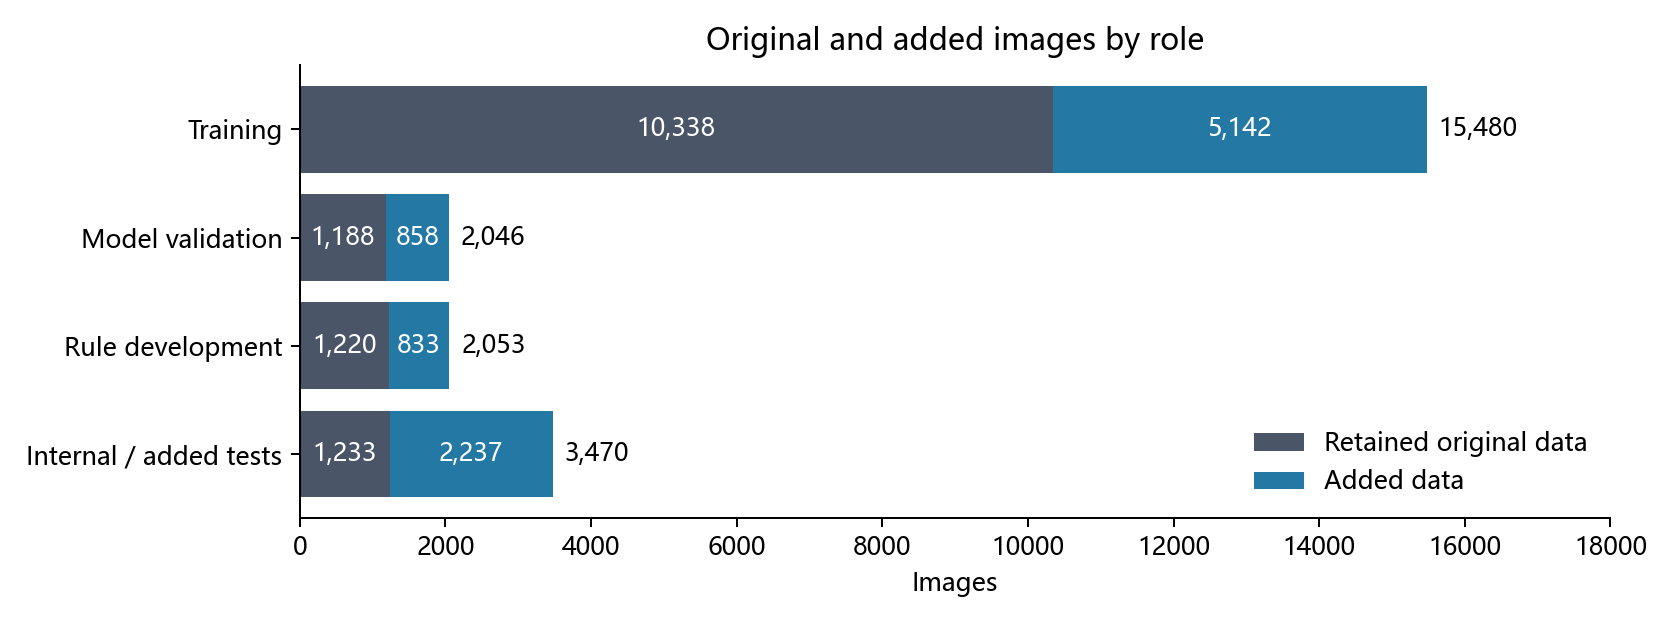
\includegraphics[keepaspectratio,alt={Original and added images allocated by role}]{cohort-allocation.en.png}}
\caption{Original and added images allocated by role}
\end{figure}

Figure 1 shows image counts in the four main roles. Of the additive
pool, 5,142 images enter training; the remainder enter model validation,
rule development, or reserved tests. The table separately lists the
1,442 ACRIMA and HYGD external-test images.

\subsection{Experimental comparison}\label{experimental-comparison}

All four arms use EfficientNet-B0, the same initialization and seed
20261113, batches of up to 16 images, and 1,200 optimizer updates each.
The original-data arm uses 10,338 corrected training images; the three
expanded arms use 15,480. Expanded data are combined with 0\%, 30\%, or
50\% probabilities of mixed degradation, covering uneven illumination,
defocus, and scattering. Degradation augments disease training;
quality-model targets remain tied to original images.

Models are evaluated every 300 updates on the same 2,046
model-validation images. The original selection rule averages AUROC
equally over 11 sources with both classes. The original-data, 30\%, and
50\% arms select update 1,200; expanded data without degradation selects
update 300. The comparisons below use update 1,200 for every arm to
align training budgets.

\subsection{Observed results}\label{observed-results}

AUROC stands for ``area under the receiver operating characteristic
curve.'' Changing the disease-score threshold produces different
sensitivities (the proportion of positives detected) and false-positive
rates (the proportion of negatives classified as positive). The ROC
curve plots their relationship, and AUROC measures the area beneath it.

AUROC also represents the probability that a randomly selected positive
image receives a higher score than a randomly selected negative image,
counting ties as half. An AUROC of 0.93 means this ranking probability
is about 93\%; 0.5 corresponds to random ranking and 1.0 to perfect
separation. Actual misses and false positives are evaluated at a chosen
threshold. The following results use original photographs from the same
rule-development set, calculated separately within each source.

{\def\LTcaptype{none} % do not increment counter
\Needspace{8\baselineskip}
\begin{longtable}[]{@{}lrrrr@{}}
\toprule\noalign{}
Source & Original & Expanded & 30\% degradation & 50\% degradation \\
\midrule\noalign{}
\endhead
\bottomrule\noalign{}
\endlastfoot
AIROGS & 0.9687 & 0.9551 & 0.9583 & 0.9593 \\
ODIR & 0.9712 & 0.9315 & 0.9281 & 0.9404 \\
LAG & 0.9465 & 0.9890 & 0.9844 & 0.9832 \\
KEH & 0.6627 & 0.9333 & 0.9321 & 0.9368 \\
\end{longtable}
}

Development images / positives are AIROGS 773 / 380, ODIR 305 / 28, LAG
481 / 169, and KEH 153 / 75.

Expansion increases AUROC by 0.2706 on KEH and 0.0425 on LAG. Their 95\%
intervals from 4,000 paired resamples of linked groups are {[}0.1818,
0.3639{]} and {[}0.0248, 0.0616{]}. AIROGS and ODIR decrease by 0.0136
and 0.0397, with both intervals below zero. These intervals describe
development-case sampling uncertainty; this round uses one training
seed.

Stress evaluation creates defocus and reduced-exposure variants of a
fixed subset of 384 rule-development originals: 146 positives and 238
negatives. Under defocus, 50\% degradation improves AUROC from 0.8894 to
0.9449 relative to expanded data without degradation. At threshold 0.5,
false positives fall from 68/238 to 19/238 and misses rise from 18/146
to 28/146. Reduced false positives and increased misses also occur when
source thresholds set on model validation are held fixed.

\begin{figure}[H]
\centering
\pandocbounded{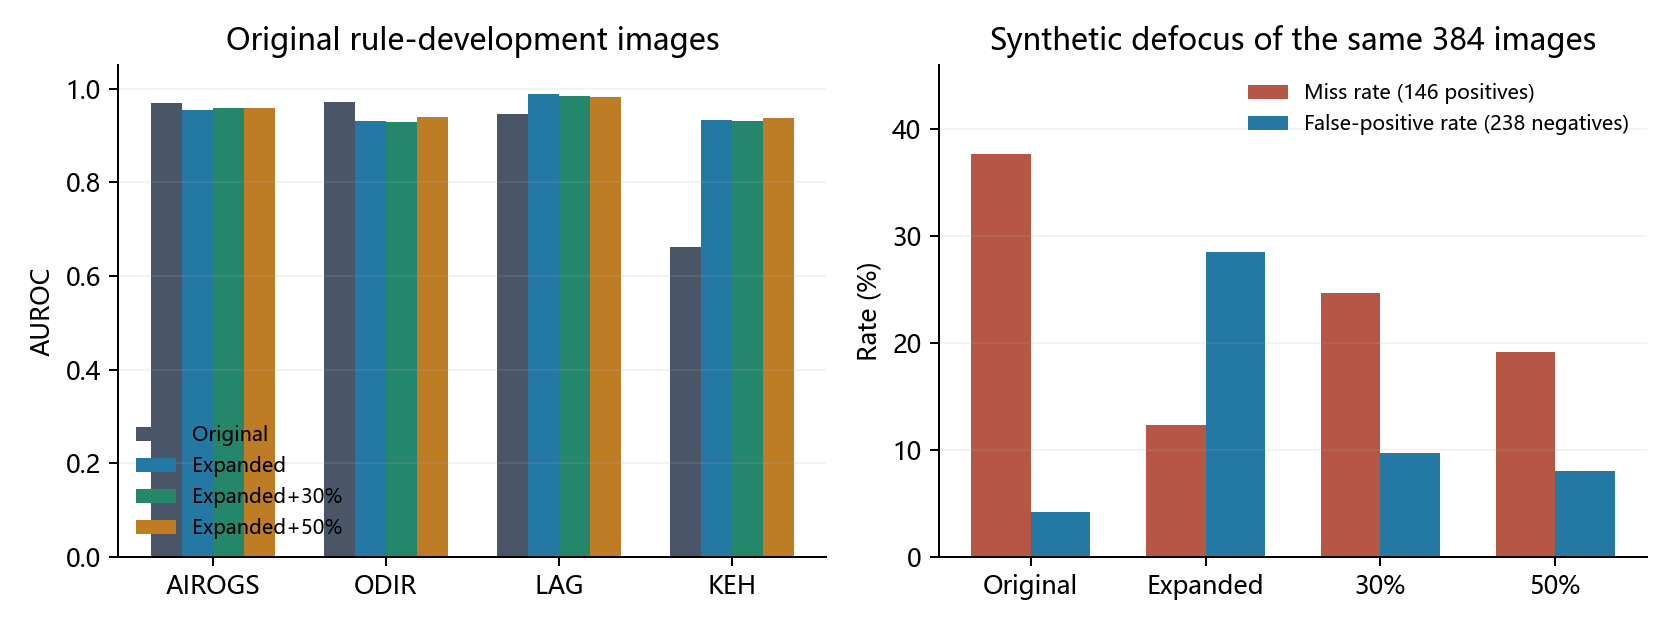
\includegraphics[keepaspectratio,alt={Source ranking and synthetic defocus results at update 1200}]{experiment-overview.en.png}}
\caption{Source ranking and synthetic defocus results at update 1200}
\end{figure}

Figure 2 shows original-image AUROC for four sources on the left and
miss and false-positive rates on the same defocus subset at threshold
0.5 on the right. The two rates use positive and negative image counts
as their respective denominators. Ranking, misses, and false positives
jointly describe the effect of degradation augmentation.

Real poor-quality development cases comprise seven FIVES and five MSHF
positive images. At threshold 0.5, original-data training detects 7/12
and all three expanded arms detect 12/12; the binomial 95\% interval for
12/12 is 73.5\%--100\%. All images in this subset are positive, and
detection counts are identical across the expanded arms. The observed
real poor-quality detection gain therefore accompanies data expansion.
Same-source negatives are needed to assess false positives.

\subsection{Disease and quality score
distribution}\label{disease-and-quality-score-distribution}

The figure matches disease score p from the update-1,200 checkpoint of
the 50\% mixed-degradation arm with raw regression score q from the
previously verified FTHNet-distilled quality student. It covers 1,220
retained original rule-development images (503 positive and 717
negative). Higher q indicates better predicted quality; it is neither a
human quality grade nor a calibrated probability. The 833 added
development images do not yet have verified scores from this same
quality model and are excluded.

\begin{figure}[H]
\centering
\pandocbounded{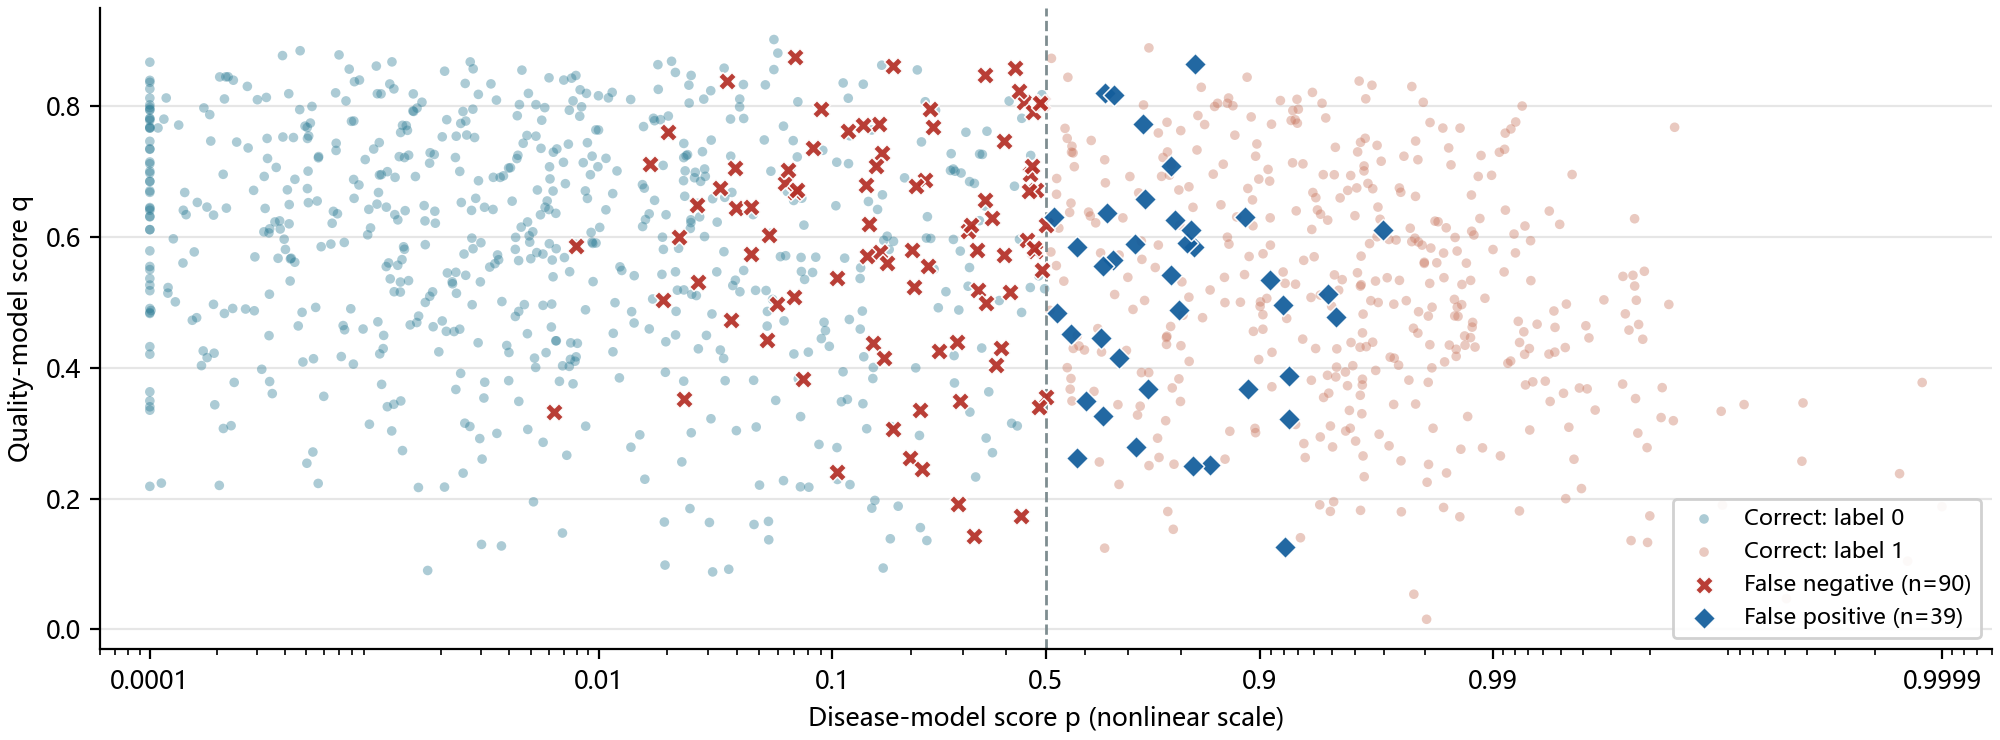
\includegraphics[keepaspectratio,alt={Disease and quality scores on original rule-development images}]{pq-distribution.en.png}}
\caption{Disease and quality scores on original rule-development images}
\end{figure}

Figure 3 uses a nonlinear horizontal axis for disease score p and a
vertical axis for quality score q. Pale circles show correct
predictions; red crosses highlight false negatives, and blue diamonds
highlight false positives. For display, p is clipped to 0.0001--0.9999.
At the illustrative threshold of 0.5, marked by the dashed line, there
are 90 misses among 503 positives and 39 false positives among 717
negatives. Correct predictions remain visible to show how many might
also fall in a potential review region. This threshold is illustrative,
and no review boundary has been selected. The
\href{pq-distribution.json}{figure data} contain counts and errors in
linear p and q bins, together with input hashes; see also the
\href{../../../tools/plot_pq_overview_20261113.py}{plotting program}.

\subsection{Priorities identified by the
analysis}\label{priorities-identified-by-the-analysis}

After expansion, original-source image presentations fall from 19,186 to
9,484; all three expanded arms have the same image-sampling sequence.
Adaptation to added sources and reduced original-source sampling occur
together. The next round will use an original-source sampling quota to
separate their effects.

HRF, CRFO, Fundus-AVSeg, and LES-AV contribute only 15 validation images
but account for four equally weighted sources, or 36.4\% of the current
checkpoint-selection mean. Ranking changes in a few images can therefore
strongly affect checkpoint choice. The proposed next round uses AIROGS,
ODIR, Kaggle, LAG, and KEH as primary selection sources, saves every
validation checkpoint, and compares three common seeds at a budget of
2,400 updates.

Training quality annotations are strongly associated with disease class.
Further work will add real poor-quality negatives, compare defocus-only
and mixed augmentation, and set classification thresholds on
model-validation data. Model selection and manual-review rule
development will precede evaluation on reserved tests. The
\href{experimental-analysis/experimental-analysis.en.md}{statistical
analysis} and \href{../../operations/next-steps.en.md}{next-steps
checklist} describe the proposed comparisons.

\subsection{Relationship to earlier training and
evidence}\label{relationship-to-earlier-training-and-evidence}

The earlier \texttt{formal\_v3} disease models, original quality model,
and \texttt{eyeq\_quality\_v1} each completed 20 epochs. The November 12
report records disease checkpoints selected at epochs 16 and 18, with
AIROGS model-validation AUROCs of 0.9766 and 0.9831. The selected
epoch-17 EyeQ quality checkpoint achieved three-grade macro-F1 0.811 on
117 EyeQ validation images. This round uses a new data release and
expanded evaluation sets; the two rounds have separate interpretations.

Evidence includes
\href{../../../data/prepared/expanded_20261113/cohort_verification.json}{frozen-cohort
verification},
\href{../../../runs/expanded_20261113/budget_end_comparison.json}{update-1,200
results}, \href{experimental-analysis/analysis.json}{paired statistics},
and the
\href{../../../tools/build_progress_overview_20261113.py}{overview build
program}. Image-level predictions, full logs, datasets, and weights
reside in local data and run directories. Report tables, figures, and
statistical summaries are saved with the repository.

\end{document}
